

Para obtener información de forma más rápida y poder comparar fácilmente las características 
de los tres sistemas se ha usado el portal \href{https://db-engines.com/en/system/MongoDB\%3BPrometheus\%3BRedis}{DB-engines.com}. 
La siguiente tabla contiene las características principales de cada uno de ellos. Esta información
solo tiene carácter orientativo y será contrastada a la hora de tomar una decisión de diseño

% \begin{figure}
%     [Tabla bases]
%     {FIG:MONGO_VS_RD33BMS}
%     {Tabla bases}
%     \pgfimage[10cm]{tabla_comparativa_bases_de_datos.pdf} 
%     %\image{}{}{tabla_comparativa_bases_de_datos}
% \end{figure}

% Solución temporal. Puede quedar mejor usando figuras
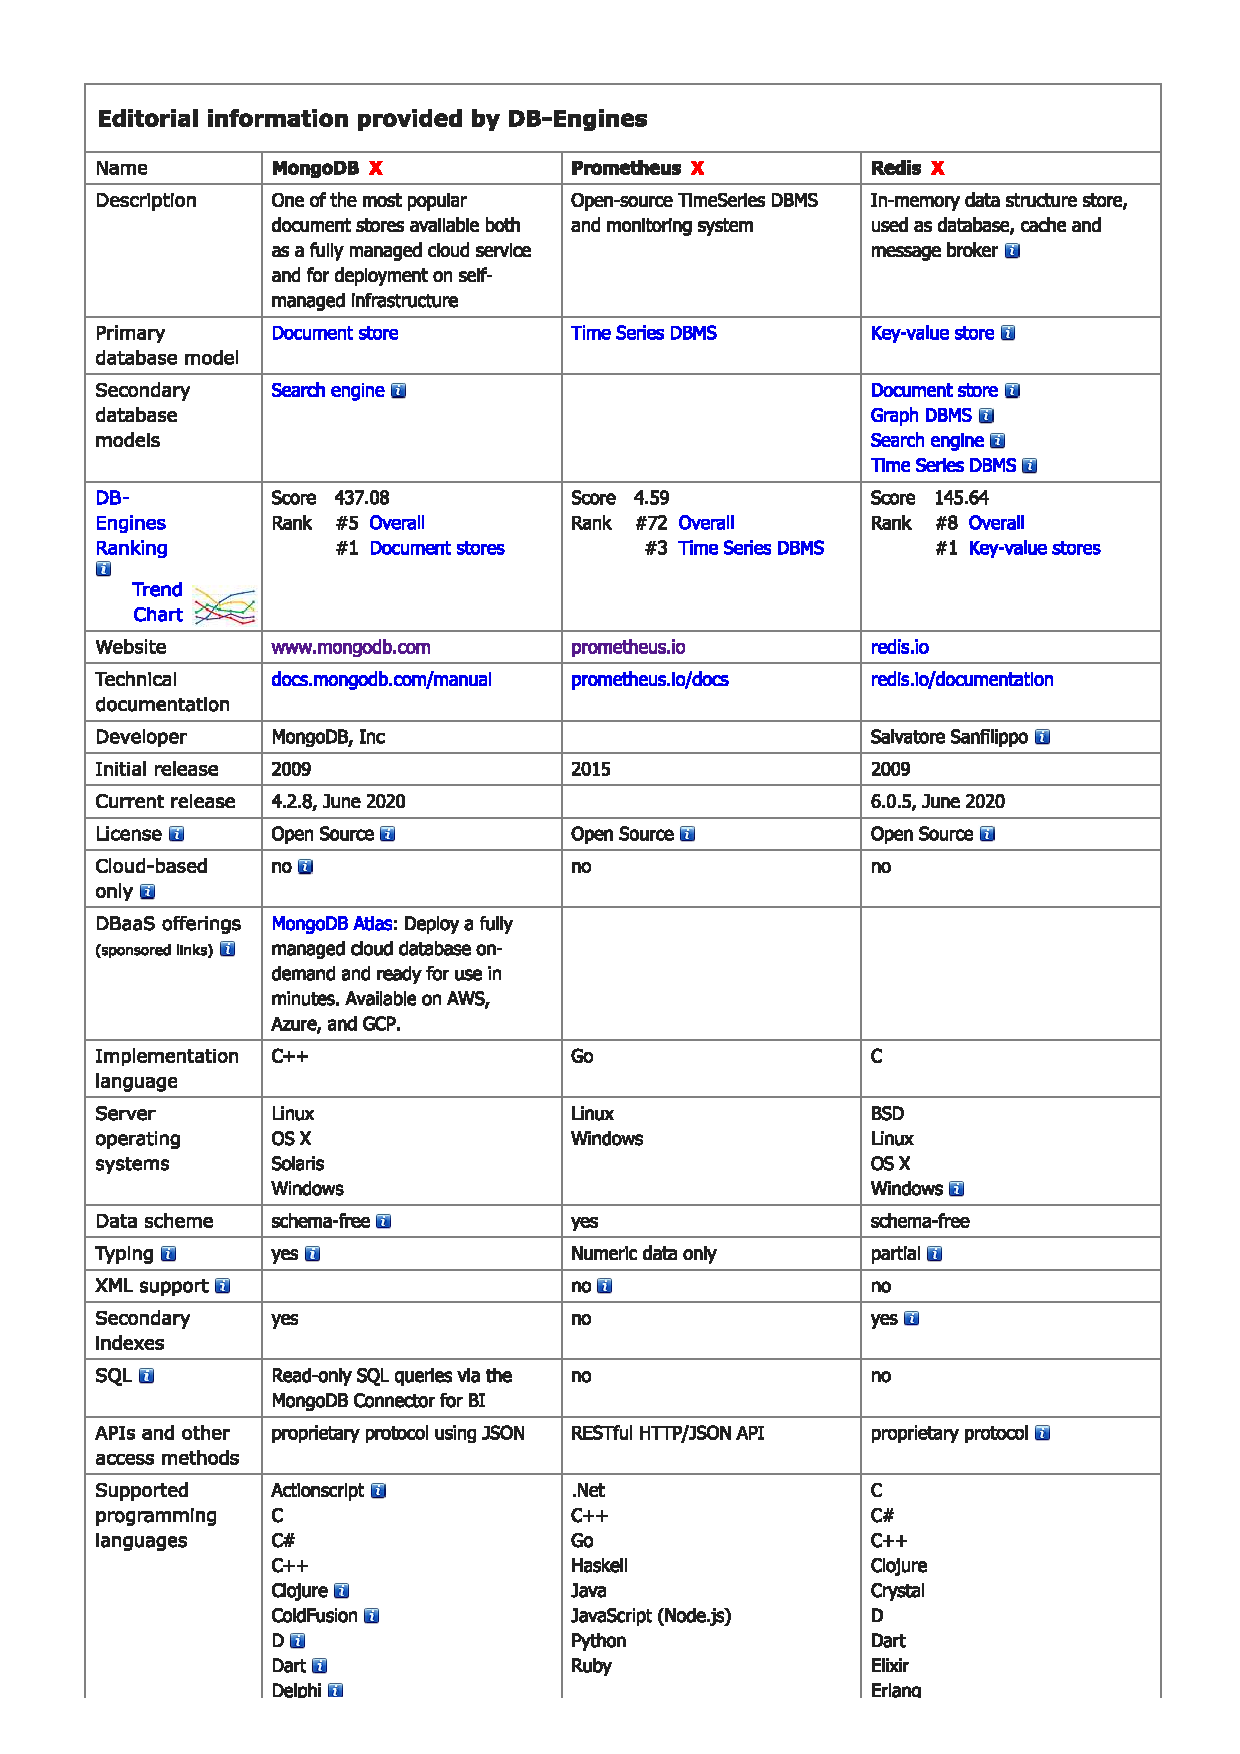
\includepdf[pages=-]{graphics/tabla_comparativa_bases_de_datos.pdf}